\documentclass[11pt]{article}
\usepackage{lac2005}
\usepackage{graphicx}
%\usepackage{a4}
\usepackage[latin1]{inputenc}
\sloppy
\newenvironment{contentsmall}{\small}

\title{Ontological Processing of Sound Resources}

\author
{J�rgen Reuter
% \\ Group, Lab, Organisation 
% \\ Luwdig-Windthorst-Str. 11
% \\ 76187 Karlsruhe,
\\ Karlsruhe, Germany,
\\ http://www.ipd.uka.de/\~{}reuter/ }


\begin{document}
\maketitle


\begin{abstract}
\begin{contentsmall}
Modern music production systems provide a plethora of sound resources,
e.g.\ hundreds or thousands of sound patches on a synthesizer.  The
more the number of available sounds grows, the more difficult it
becomes for the user to find the desired sound resource for a
particular purpose, thus demanding for advanced retrieval techniques
based on sound classification.  This paper gives a short survey of
existing approaches on classification and retrieval of sound
resources, discusses them and presents an advanced approach based on
ontological knowledge processing.
\end{contentsmall}
% 84 words
\end{abstract}

\keywords{
\begin{contentsmall}
classification of sounds, sound resource lookup, ontologies, OWL
\end{contentsmall}
}

% TODO: Introductory scenario; e.g. looking for particular sound
% TODO: add ref to multimodal paper

\section{Introduction}

State-of-the-art music production systems consist of a
computer-centered, heterogeneous network of hardware and software
modules with typically huge banks of sound resources.  Modern hardware
synthesizers or tone modules often have banks with hundreds or
thousands of different sounds. Producing electronic music therefore
means to select among synthesizer or tone modules, as well as to
select sounds from each module.  Modules not only (if at all) provide
factory presettings, but typically also reserve much memory space for
lots of user patches that may be tweaked manually or loaded via MIDI,
thereby even increasing the number of available sounds.  The music
producer's task of selecting a sound thus becomes an increasingly
complex challenge.

For example, imagine a composer who has already in mind a vague idea
of the electronic sounds that should be used for a new piece of music.
In an older piece a couple of years back in time, there was a bass
line with a bass sound that also should fit well for the new piece.
But what synthesizer was used to produce this sound?  Even if the
synthesizer is known, which one of the hundreds or thousands of sound
patches was used?  If it was a user patch, where was the patch stored?
Even if the sound can be located, over which specific MIDI port and
channel can the sound be addressed?  Unfortunately, on many
synthesizers, sound patches are ordered in a fairly chaotic fashion,
especially, if they do not fit into the GM sound map.  In the worst
case, the composer has to scan through thousands of sound patches to
find the desired one.  What is required, is the possibility to search
for a particular sound.

Searching for a file in a file system is conceptually fairly straight
forward, given the name of the file (or part of it), or the file type,
or some content that is known to appear in the file.  In contrast,
searching for a sound is much more challenging.  First of all, while
all files in a file system can be iteratively accessed by browsing
through the directory hierarchy, there is, as of this writing, no
central registry for all sound resources that are available on the
system.  Rather, every synthesizer has its own approach of managing
sound patches.  Secondly, while files can be searched for by their
name or type or content, defining useful search criteria for sounds is
difficult.  Finally, searching for near matches means to have a system
that allows for defining proper metrics of sound comparison.

In the above example of looking for a bass sound, listing all
available bass sounds would already fairly reduce the number of sound
resources that have to be further checked.  If the bass sound can be
qualified even more specific, the search could be even more effective.
In this article, we examine and discuss multiple approaches for
classifying and describing sounds.  We present a prototype design and
implementation of a sound classification and description framework
based upon ontological technology.  We show how this framework enables
us to search for specific sounds.  Finally, we discuss the impact of
further pursuing this approach on Linux audio development.

% * lots of synths with hundreds or thousands of sound patches
% * each synth has its own GUI, philosophy/concept of sythesis and use
% * on which synth was that cool string pad sound?
% * ok, I accidentally remember it's on synth xyz, because I used it
%   in a project abc that was produced with synth xyz
% * on which Port / MIDI channel can I address synth xyz?
% * how do I find the sound on synth xyz?

\subsection{Preliminaries}
% The Notion of the Term \emph{Sound}

%For the remainder of this article, we denote with the term
%\emph{sound} a broadened semantics, which differs from the classical
%definition.
%
%The classical definition of the term considers the shape of a periodic
%function that represents the acoustic signal (e.g.\ air pressure).
%With respect to its electric representation in analog electronic
%circuits (but neglecting any effects of quantum physics), such a
%function can be assumed to be continuous, limited, and with limited
%slope (due to limited signal bandwidth).  Without loss of generality,
%the period can be normalized to a specific value (e.g.\ $2\pi$), when
%the actual pitch of the sound is irrelevant.  To ensure that the
%period represents the base frequency of the sound, one may further
%demand that it is not a sequence of a repeated subperiod (unless the
%function is constant in which case there is no base frequency).  If it
%is, the subperiod has to be taken as the actual period.  Furthermore,
%the function may be normalized with respect to its amplitude by
%multiplying it with a constant, such that the maximum elongation
%equals 1.  Given such a periodic function, it is easy to see that a
%fourier series can be computed from it.  The series of fourier
%coefficients then represents a series of partial tones that fully
%characterize the sound.  In theory, this series is infinite; however,
%assuming limited bandwidth, the coefficients beyond the supported
%frequency range are irrelevant.  Thus, in the sense of the classical
%notion of the term, a bandwidth-limited sound can be fully
%characterized by a finite series of fourier coefficients, that
%represents the harmonic spectrum of the sound.

There is a mismatch between the classical, rather mathematical notion
of the term sound and the common conception of sound as viewed by most
musicians and music listeners.  While the classical definition solely
focuses on the core wave shape of a periodic signal, most people
perceive aperiodic characteristics also as part of a sound.  Among
such aperiodic characteristics are vibrato, noise content, reverb or
echo content, but also irregularities of the harmonic spectrum such as
non-equidistant partials or partials that vary in pitch or amplitude.
For the remainder of this article, we therefore extend the classical
definition by also incorporating such aperiodic properties into the
notion of sound.

\subsection{Paper Outline}
We start with a short survey of how various systems currently address,
if at all, the sound selection problem (Section \ref{related_work}).
Then we discuss the approaches in order to reveal commonly used
strategies (Section \ref{discussion}).  Based upon this discussion, we
develop an ontological framework in order to solve the sound selection
problem in a unified way (Section \ref{sound_resources_ontology}).  We
demonstrate the usefulness of our system by giving some examples of
how the user can benefit from the system (Section \ref{evaluation}).
%Recent scientific findings in the field of synaesthesia suggest
%directions for future investigation in this field (Section
%\ref{future_work}).
The work presented here has a significant impact on Linux audio
development in general and on construction of software synthesizers in
particular, which is left for further investigation (Section
\ref{future_work}).  We complete our journey with a concluding summary
of our results (Section \ref{conclusion}).

\section{Related Work}
\label{related_work}

We give a short survey on the history of sound classification, from
acoustic instrument taxonomies and organ disposition over grouped
categories in the MIDI standard to what recent synthesizers provide.
This survey is not at all meant to be complete, but establishes some
central ideas for sound classification that we will discuss and
further develop in the subsequent sections.

\subsection{Instrument Taxonomies}
\label{instrument_taxonomies}

Classification of acoustic instruments has a long tradition.  Figure
\ref{instrument_taxonomy} shows an example taxonomy of selected
acoustic instruments as it can be found in this or similar form in
standard music literature.  Note that such taxonomies are typically
based on how an instrument technically \emph{works} rather than how it
\emph{sounds}.  Still, if two instruments work similarly, they often
sound similarly.  Eventually, however, a small change in construction
may result in a tremendous change in sound. %%% TODO: example

\begin{figure}[htb]
  \centering \leavevmode
  \includegraphics[angle=0,width=0.48\textwidth]{images/instrument_taxonomy.eps}
\caption{A Taxonomy of Selected Acoustic Instruments}
\label{instrument_taxonomy}
\end{figure}

Also note, that, traditionally, the realization of the sound source of
the instrument is more important for classification than e.g.\ that of
the body.  For example, a saxophone has a reed mouthpiece and
therefore is considered to be a reed instrument regardless of its
metallic body, while the so-called Indonesian trumpet is blown like a
trumpet and therefore considered as brass instrument, regardless of
its wooden body.

\subsubsection{Dispositional Approach}

The situation is slightly different for the (acoustic or electric)
organ, which has the ambition of uniting many instruments (organ
registers) into a single apparatus.  While, at least for the acoustic
organ, there is also a technical classification of pipes based on how
they \emph{work} (e.g.\ labial or stopped pipes), organ registers are
often named after well-known acoustic instruments (e.g.\ flute,
trumpet, saxophone), i.e. how they \emph{sound}.  Indeed, the organ's
naming of registers is maybe the oldest example for a categorization
of sounds: it assists the organ player in looking up a sound.  This is
especially important since each organ has an individual, more or less
rich set of sounds, and that way, a guest organ player can quickly get
familiar with a foreign organ.  Remarkably, already Supper\cite{S50}
notes that the rules, which underly the disposition of an organ, are
of hierarchical kind.  We will resume this idea, when presenting a
framework for describing and looking up sounds (cp.\ Section
\ref{sound_resources_ontology}).

\subsection{Grouping}
\label{gm_standard}
The instrument patch map of the General MIDI (GM) Level 1
Standard\cite{GM01} defines 128 instruments that are partitioned into
sixteen categories (cp.\ Fig.\ \ref{gm_categories}).

\begin{figure}[htb]
  \centering \leavevmode
\begin{tabular}{|l|l|}
\hline
Program & Family \\ \hline \hline
1-8 & Piano \\
9-16 & Chromatic Percussion \\
17-24 & Organ \\
25-32 & Guitar \\
33-40 & Bass \\
41-48 & Strings \\
49-56 & Ensemble \\
57-64 & Brass \\
65-72 & Reed \\
73-80 & Pipe \\
81-88 & Synth Lead \\
89-96 & Synth Pad \\
97-104 & Synth Effects \\
105-112 & Ethnic \\
113-120 & Percussive \\
121-128 & Sound Effects \\ \hline
\end{tabular}
\caption{GM Level 1 Sound Categories}
\label{gm_categories}
\end{figure}

Originally, the motivation for specifying an instrument patch map was
driven by the observation that a MIDI file which was produced on some
MIDI device sounded totally different when reproduced on a different
MIDI device because of incompatible mappings from MIDI program numbers
to sounds.  Therefore, in the early days, MIDI files could not be
easily exchanged without patching program change commands.  Hence, the
main purpose of the GM instrument patch map was to specify a fixed
mapping from MIDI program numbers to sounds.  Given the existing MIDI
devices of the time when the GM standard was created, a set of 128
prototype sounds, so-called instruments, was specified and assigned to
the 128 MIDI program numbers.  A GM compatible device has accordingly
to provide sounds that match these prototype sounds.  Still, the GM
standard explicitly leaves the specification of prototype sounds fuzzy
and thus encourages device implementors to take advantage of space for
variations of an actual MIDI device.  Hence, when playing a MIDI file
among different GM compatible devices, there will be typically an
audible difference in quality or style, but the overall impression of
the performance is expected to remain.

The GM instrument patch map specifies prototype sounds that were
popular on mainstream MIDI devices at that time.  Remarkably, most
sounds in the map represent acoustic or electro-acoustic instruments
as used in classical or popular music.  They are grouped roughly
following the classical taxonomies of instruments (cf. Section
\ref{instrument_taxonomies}).

Only the four categories \emph{Synth Lead}, \emph{Synth Pad},
\emph{Synth Effects} and \emph{Sound Effects} contain a collection of
sounds that allude to specific sounds that had evolved in electronic
music and were widely used since then.  The former two allude to a
qualitative categorization (\emph{lead}, \emph{pad}), while the latter
two (\emph{effects}) allude to the intended purpose of use.

Due to the extraordinary relevance of drum sounds in temporary music,
the GM standard also defines a drum map that assigns basically
fixed-pitch drum sounds to MIDI pitch numbers.  Having a fixed pitch
(unless pitch-bended or otherwise tuned), drums constitute a separate
category of their own.  Within this category of drums, however, there
is no further categorization perceivable, except, maybe, that those
drums that represent a standard drummer's hardware are grouped
together in the lower part of the map, while Latin percussion and
ethnic drums are mostly assigned to upper pitches.  In this sense, the
drum map itself maybe considered to be ordered according to the style
(i.e. intended use or purpose) of the drums.

\subsection{Banking}
\label{gm_multibank}
% Multi-Bank GM Mappings
More recent MIDI devices break the limit of 128 program numbers by
introducing \emph{sound banks}: with the bank select MSB/LSB
controller channel messages, a MIDI channel can be directed to switch
to a different bank of sounds.  In order to remain GM compatible, each
bank should itself conform to the GM instrument patch map, but may
provide a different style of sounds (e.g.\ ``bright'', ``resonant'',
``slow'', ``fast decay'').  Unfortunately, some manufacturers added
this way also such sounds, that do not really fit to the GM instrument
patch map.  (Not only) therefore, the GM Level 1
Guidelines\cite{GMDG98} discourage the use of banks at all on GM Level
1 compatible devices.  We put on record that adding new sounds to an
existing system of fixed categories may lead to difficulties.

\subsection{Tagging}
\label{tagging}

The Virus TI synthesizer\cite{A04} has a function for tagging each
sound patch with up to two values of a predefined set of 21 group
identifier.  These identifiers are:

\begin{figure}[htb]
  \centering \leavevmode
\begin{tabular}{|l|}
\hline
Acid
Arpeggiator
Bass
Classic
Decay\\
Digital
Drums
EFX
FM
Input
Lead\\
Organ
Pad
Percussion
Piano
Pluck\\
String
Vocoder\\
Favorites 1
Favorites 2
Favorites 3\\ \hline
\end{tabular}
\caption{Supported Tags of the Virus TI}
\label{virus_tags}
\end{figure}

By tagging a sound with one of these identifiers, the sound is
declared to be a member of a respective group of sounds.
Interestingly, if we look at the group names, we can identify exactly
the same categorization principles that we already met before:

\begin{itemize}

\item Identifiers like \emph{Acid}, \emph{Bass}, \emph{Classic},
\emph{Digital}, \emph{Drums}, \emph{Lead}, \emph{Organ}, \emph{Pad},
\emph{Percussion}, \emph{Piano}, \emph{Pluck} and \emph{String}
suggest groups based upon similarity to sounds that the user is
assumed to already know.  Note that some of the identifiers such as
\emph{Drums} or \emph{Percussion} denote a rather wide field of
sounds.

\item The identifier \emph{EFX} (for sound effects) presumably denotes a
group of sounds classified by its typical purpose (namely a sound
effect rather than e.g.\ a musical instrument).

\item Identifiers such as \emph{Arpeggiator}, \emph{Decay}, \emph{FM},
\emph{Input} and \emph{Vocoder} allude to how the sound is created.

\item The three \emph{Favorites} groups finally can be considered as
generic groups for which the user individually specifies the exact
semantics.

\end{itemize}

\subsection{Parametric Categorization}

State-of-the-art sound hardware provides sets of parameters that are
used to define sound patches by mainly specifying how to create the
sound.  This approach suggests to categorize sounds based on the
values of such parameter sets.  However, the size and structure of the
parameter sets differs widely across particular devices.

The MIDI specification defines a few controllers for controlling e.g.\
vibrato, envelope and a selected set of filters.  Most of these
controllers have post-processing characteristics, which is of interest
in particular for sample-based tone generators.  In contrast, the
parameter sets of synthesizers are typically much bigger and broader
than those of tone generators, since they affect also the core
generation of sound.  For example, synthesizers often provide complex
networks of oscillators, filters, and controllers with numerous
possibilities of parameterization.  Unfortunately, most synthesizers
have sound parameters that are specific for each device individually.
Even worse, a categorization based on large and complex parameter sets
makes the categorization itself complex.

Due to the plethora of existing methods of synthesis, it seems
doubtful that there will ever be agreement on a comprehensive standard
set of sound parameters.  Yet, more recent scientific work suggests
new parameters that look like candidates for standardization.  Maier
et.\ al.\cite{MBBBB05} characterize sounds by quantitative properties
that can be directly computed from the acoustic signal.  To describe
sounds, they compute for example the amount of disharmonic spectrum
peaks.  Conceptually somewhat related is the observation of
Nasca\cite{N05}, that in his software synthesizer ZynAddSubFX,
controlling the bandwidth of each harmonic offers a powerful approach
to create realistic, warm sounds.  Observations like those of Maier
and Nasca suggest that such parameters are good candidates for
providing a proper model of the way sounds are perceived by human
beings.

\section{Discussion}
\label{discussion}

From the survey in the previous section, we may conclude the following
observations:

Sounds may be categorized by

\begin{itemize}

\item their similarity to a prior known set of sounds.  This approach
complies with a composer's way of thinking, if the composer
qualitatively specifies sounds (e.g.\ a soft, bright, crystal sound).

\item their purpose of use.  This approach complies with a producer's
way of thinking if the producer has a targeted application of sound
(e.g.\ a phone ring).

\item the way they are created.  This approach complies with a sound
engineer's way of thinking when creating a new sound patch with his or
her favorite synthesizer (e.g.\ a square wave vibrato modulated
sawtooth sound with flanger).

\end{itemize}

Regarding the structure of categorization, we may note:

\begin{itemize}

\item Categories may have a hierarchical structure, thus creating a
taxonomy.

\item It is difficult to specify orthogonal categories.  That means,
in general a sound may be a member of multiple categories.

\item Since there are most likely always sounds remaining that do not
fall into any existing category, it is useful to have generic
categories to be specified by the user that capture the remaining
sounds.

\end{itemize}

The Virus' tagging approach may be used to associate a sound to (at
most two) categories.  However, tagging does not at all consider
categories as a hierarchy, unless we support \emph{deductive} tags:
Assume, that we consider all drum sounds to be percussive.  Then, if a
sound is tagged ``drum'', it should implicitly also be tagged
``percussive''.  This way, we may specify a hierarchy of tags.  The
hierarchical taxonomy of acoustic instruments is a good candidate for
creating a hierarchy of tags.

\section{The Sound Resources Ontology}
\label{sound_resources_ontology}

Similar to the Virus TI, we follow the approach of tagging sounds with
tags that aim to characterize qualitative attributes of the sound.
For a tagging-only description and looking up of sounds, a simple
relational database approach is sufficient.  However, we would like to
group sounds in a hierarchical manner and potentially give tags a
deductive semantics as described in the previous section.  Therefore,
we prefer a framework with deductive capabilities based on ontological
technologies.

\subsection{OWL Knowledge Bases}

Ontologies are an appropriate means for describing hierarchical
structures of \emph{classes of individuals} (also called
\emph{concepts}) in a flexible way, based on description logic.  The
\emph{Web Ontology Language OWL}\cite{MH04} with its three
sub-languages \emph{OWL-Full}, \emph{OWL-DL} and \emph{OWL-Lite} has
emerged as the maybe most important standard for description logic
languages.  For the remainder of this article, we consider OWL-DL,
which specifies description logic semantics that is a decidable
fragment of first-order logic.  In contrast to \emph{rule-based logic}
such as Prolog or Datalog, the \emph{description logic} of OWL-DL
focuses on features such as hierarchical concepts, \emph{properties}
(i.e. binary relations between pairs of individuals or an individual
and a data value), and property and cardinality \emph{restrictions}.
OWL can be expressed in XML-based \emph{RDF}\cite{MSB04} syntax, which
we use as source file format.  The entire ontological description,
regardless whether stored in memory or on disk, and regardless in
which language specified, is usually referred to as the so-called
\emph{knowledge base}.  Similar to a database, a knowledge base
typically may be updated, and its current content may be queried (cp.\
Fig.\ \ref{knowledgebase}).
% TODO: explain facts knowledge

\begin{figure}[htb]
  \centering \leavevmode
  \includegraphics[angle=0,width=0.48\textwidth]{images/knowledgebase.eps}
\caption{Updating and Querying an OWL Knowledge Base}
\label{knowledgebase}
\end{figure}

The initial knowledge base is created from a file specified in RDF.
The current version is available at:
\texttt{http://www.ipd.uka.de/\~{}reuter/
ontologies/lad/sound/sound-registry.owl}

\subsection{Ontology Design}

Following the discussion in Section \ref{discussion}, our ontology
contains a concept \texttt{Sound} that serves as common super class
for all particular sounds.  Respecting the categories of GM Level 1
devices, our ontology defines a subclass \texttt{GMSound} that
disjointly divides into the 16 GM categories, each represented by a
concept of its own.  At the same time, \texttt{GMSound} also divides
into (generally overlapping) groups that correspond to the different
\texttt{SoundQuality} individuals.  Each \texttt{SoundQuality}
individual represents a tag of those in Fig.\ \ref{virus_tags} or of a
few others, that have deliberately been added, inspired by the GM
categories.  That way, we basically have two independent hierarchies
of sounds, thus giving the user more choices in querying or browsing
for a particular sound.  The ontology also features a concept
\texttt{SoundResource}.  Each individual of this class represents a
resource that hosts \texttt{Sound} individuals.  An example for a
\texttt{SoundResource} individual is a particular MIDI synthesizer.
The ontology also models a \texttt{SoundPort} concept with the
subclass \texttt{ALSAPort} such that for each \texttt{SoundResource}
individual, a port can be looked up in order to access the resource.
A \texttt{SoundSubscriber} finally may allocate any number of
\texttt{Sound} individuals, such that the number of available sounds
left can be tracked.
%Fig.\ \ref{concept_hierarchy} gives an impression of the complete
%hierarchy of concepts.
Property constraints are deployed to bind GM sounds to MIDI program
numbers.

\section{Evaluation}
\label{evaluation}

To demonstrate the usefulness of our approach, we walk through a short
sample tour on exploring the space of sounds, using \emph{The Prot�g�
Ontology Editor and Knowledge Acquisition System}\cite{CMNR05} for
visualization (cp.\ Fig.\ \ref{protege_overview}).  This free, open
source application from Stanford University provides a graphical user
interface for viewing and editing ontologies.  Note that there are a
lot of OWL related tools on the net\cite{MH04}; in this section, we
just use Prot�g� for illustration purposes.  One could also take some
OWL reasoner with API, for example Jena \cite{HP05}, and develop
appropriate command line tools or dedicated interactive applications
for exploring the space of sounds.  However, in this section we chose
Prot�g� for the purpose of illustrative visualization.

\begin{figure}[htb]
  \centering \leavevmode
  \includegraphics[angle=0,width=0.48\textwidth]{images/protege-overview.eps}
\caption{The Sound Registry Ontology viewed with Prot�g�}
\label{protege_overview}
\end{figure}

\subsection{Querying for a Sound}

We start querying for a sound by specifying properties that the sound
must fulfill.  In the illustrated example (Fig.\
\ref{protege_query_part1}), we ask for a sound that fulfills the two
sound qualities ``Synth'' and ``Bass'' and, additionally, lives on the
``MU-50'' sound resource.  Note that properties have a well-defined
domain and range, such that Prot�g� lets us select e.g.\ the sound
quality only from the actual list of available sound qualities (rather
than accepting any arbitrary individual or data value).

\begin{figure}[htb]
  \centering \leavevmode
  \includegraphics[angle=0,width=0.48\textwidth]{images/protege-query-part1.eps}
\caption{Querying for a Sound on the MU-50 with ``Synth'' and ``Bass''
Qualities}
\label{protege_query_part1}
\end{figure}

Prot�g� returns a result consisting of three sounds that match our
constraints (Fig.\ \ref{protege_query_part2}).  We find the
``Generic-GM-BassAndLead'' sound most interesting and double-click on
it to find out more about it.

\begin{figure}[htb]
  \centering \leavevmode
  \includegraphics[angle=0,width=0.48\textwidth]{images/protege-query-part2.eps}
\caption{The Search Results}
\label{protege_query_part2}
\end{figure}

A proper window pops up (cp.\ Fig.\ \ref{protege_query_detail1}).  In
this window we can see that the sound indeed fulfills our three
constraints.  Moreover, we learn to know that this sound maps to MIDI
program 88.  Imagine that we were not using Prot�g�, but a dedicated
application embedded e.g.\ into a sequencer software; then the
software could exploit the MIDI channel value to, for example, set the
MIDI program of the currently selected track.  We also notice the
\texttt{rdfs:comment} field with a detailed annotation regarding this
sound.  Finally, in the field \texttt{hasQuality}, we can see, that
this sound not only fulfills the qualities ``Synth'' and ``Bass'' as
required in our query, but also the quality ``Lead''.  In order to
look, what this quality means, we double-click on ``LeadQuality''.

\begin{figure}[htb]
  \centering \leavevmode
  \includegraphics[angle=0,width=0.48\textwidth]{images/protege-query-detail1.eps}
\caption{Viewing the Generic GM ``Bass And Lead'' Sound Properties}
\label{protege_query_detail1}
\end{figure}

Again, a proper window pops up (cp.\ Fig.\
\ref{protege_query_detail2}).  This window shows a description of the
``Lead'' quality in the field \texttt{rdfs:comment}, such that we
learn to know even more characteristics of the sound than what we
actually required in our query.

\begin{figure}[htb]
  \centering \leavevmode
  \includegraphics[angle=0,width=0.48\textwidth]{images/protege-query-detail2.eps}
\caption{Viewing the ``Lead'' Sound Quality Properties}
\label{protege_query_detail2}
\end{figure}

\subsection{Browsing the Hierarchy of Sounds}

Searching for sounds is also possible by just browsing through the
concept hierarchy.  Prot�g� displays the concept hierarchy as a tree
that can be expanded or collapsed at your choice (cp.\ Fig.\
\ref{protege_class_browsing}).  Note that, due to possible multiple
inheritance of concepts in OWL, a concept may appear multiple times in
the tree.  For example, the \texttt{GMOrganSound} concept appears two
times in the tree, once as subclass of \texttt{GMSound}, and another
time as subclass of \texttt{OrganSound}.  Individuals of the concept
\texttt{Sound} appear on the leaf nodes of the tree and can be viewed
in more detail when selecting the appropriate leaf.

\begin{figure}[htb]
  \centering \leavevmode
  \includegraphics[angle=0,width=0.48\textwidth]{images/protege-class-browsing.eps}
\caption{Browsing through the Concept Hierarchy of Sounds}
\label{protege_class_browsing}
\end{figure}

\section{Future Work}
\label{future_work}

Our prototype ontology focuses on the description of a generic GM
Level 1 device as an example sound resource.  While we provide a
general ontological framework for virtually any kind of sound
resource, we currently do not provide a description of any specific
sound resource.  The task of providing ontological descriptions for
individual sound resources remains open for discussion.  After all,
ontological descriptions are desired for both, external hardware
synthesizers as well as software synthesizers running under Linux.
This work is in particular meant to initiate discussion on and
fostering the development of proper standards.

\subsection{Impact on ALSA Developers}

The ontological description should be accessible to virtually all
users of the audio infrastructure.  Since ALSA\cite{ALSA06} has
established as the default sound architecture on most current Linux
distributions, responsibility for provision and maintenance of the
ontological description as well as a for providing a query and
management API should probably fall to ALSA.  ALSA developers may want
to develop and establish a proper infrastructure and API.  In fact,
ALSA developers could try to standardize the ontological framework as
well as the query and management API in an interoperable manner.
Ontological descriptions could then be provided independently of a
particular operating system.  This way, ALSA developers could pave the
way for manufacturers of external hardware starting to provide
ontological descriptions of their hardware's sound resources by
themselves.  All operating systems would greatly benefit from such a
development.

\subsection{Impact on Linux Audio Application Developers}

Just like external hardware providers, developers of software
synthesizers under Linux should provide ontological descriptions of
their synthesizers' sound resources, following the standards to be
provided by ALSA developers.

Editing sound patches typically will affect the ontological
description.  For example, given a software synthesizer that lets the
user create new sounds, the software could enable the user to describe
the sound with tags, e.g.\ by displaying check-boxes or a multiple
selection list with items for each tag.  ALSA developers may want to
standardize a default set of tags.  Given such tags and other user
settings, the software synthesizer should be capable of generating on
the fly a corresponding ontological description of the sound.

If Linux audio developers feel that it is of too much burden for
software synthesizers to create ontologies, ALSA developers may
alternatively develop a sound resource query API, that each software
synthesizer should implement.  The ontological description of all
software synthesizers could then be created and managed completely by
ALSA.

\section{Conclusion}
\label{conclusion}

We showed that in complex systems with a plethora of sound resources,
characterizing sounds e.g.\ by classification is an essential task in
order to efficiently look up a particular sound.  Our historical
survey on sound classification elucidated the importance of this task.

We have demonstrated the feasibility of deploying ontological
technology for describing and looking up sounds and sound resources.
We developed a terminological knowledge base that serves as an
ontological framework, and we created a generic GM Level 1 device as
facts knowledge that serves as an example on how to use our framework.

While we focus on the technical realization of the OWL-DL based
framework, so far we leave open how to integrate this framework into
the operating system.  If Linux audio developers feel that looking up
sounds and sound resources is worth being solved in a uniform way
under Linux, further discussion on the integration with applications,
ALSA and maybe other parts of the operating system will be required.

\bibliographystyle{acl}
\bibliography{lac2006_ontology}

%\begin{figure}[htb]
%  \centering \leavevmode
%  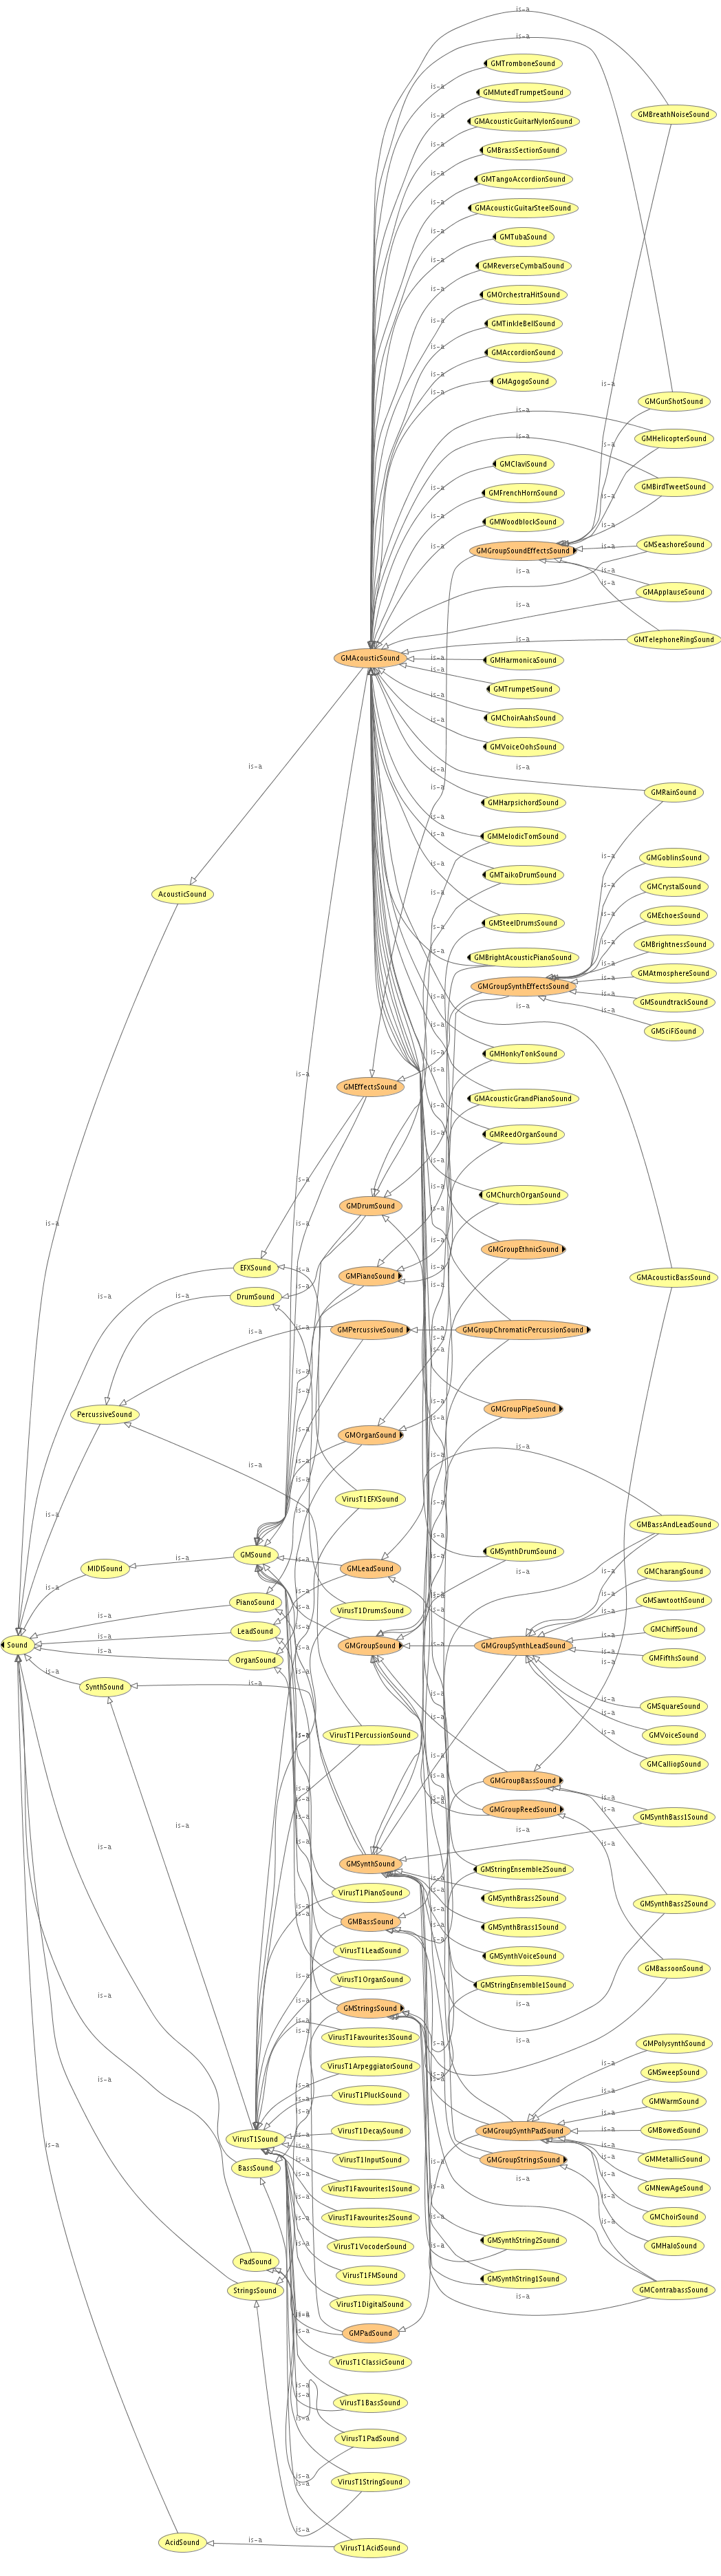
\includegraphics[angle=0,height=0.96\textheight]{images/sound-hierarchy.eps}
%\caption{Concept Hierarchy of Sounds}
%\label{concept_hierarchy}
%\end{figure}

\end{document}
